\chapter[Nível de Programa]{Nível de Programa}

\section{Requisitos Identificados}

\textbf{\textit{Feature} 01 - Listagem de contato de possíveis clientes}

Nesta \textit{feature}, espera-se obter uma lista de contatos oriúnda de registros, fornecendo portanto a oportunidade de edição e visualização de todos os contatos, assim como seus respectivos atributos e desejos.



\textbf{\textit{Feature} 02 - Padronização da divulgação dos serviços}

A partir de tal \textit{feature}, há o objetivo de incluir um padrão de apresentações para melhor abordar os clientes. Com isso, um ponto a ser agregado é a forma com que os emails serão enviados além de fornecer a visualização dos serviços que serão oferecidos pela empresa no presente período de tempo.



\textbf{\textit{Feature} 03 - Acompanhamento do contato com o cliente}

O objetivo da \textit{feature}, é trabalhar com a criação de círculos para com o cliente. Isso vai envolver o oferecimento dos serviços e de uma cartilha com as propostas. Além desse cenário favorável, deve-se registrar os clientes que rejeitaram a proposta em um primeiro momento e anotar seu \textit{feedback}, caso haja.
		



\textbf{\textit{Feature} 04 - Acompanhamento das reuniões com o cliente}

Nesta \textit{feature}, espera-se fazer todo o tratamento que envolve as reuniões, desde o planejamento da mesma, no que se refere as datas e locais das mesmas assim como a pauta do que será falado, até uma geração de relatórios do que foi debatido na mesma.		



\textbf{\textit{Feature} 05 - Controle das informações referentes ao projeto}

Se busca obter a partir de relatórios, o que de fato esta sendo realizado no projeto, se esta sendo feita da melhor maneira. Há opções capazes de realizar registros de novos projetos, custos, pessoas envolvidas, avaliar se o projeto é de fato viável etc.



\section{Visão}

\section{\textit{Roadmap}}

O \textit{Roadmap} definido juntamente com o PM encontra-se na Figura \ref{roadmap}.

\begin{figure}[!htb]
\centering
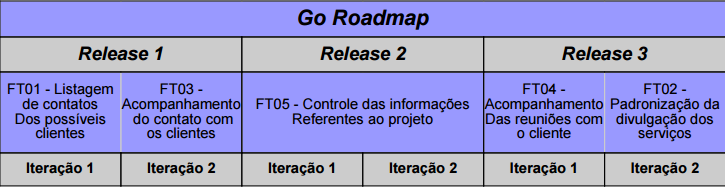
\includegraphics[scale=0.6]{figuras/roadmap.png}
\caption{\textit{Roadmap} do projeto}
\label{roadmap}
\end{figure}

\section{Planejamento da \textit{Release}}